%% ============================================================================
%% Paper 3: Quantum-Inspired Molecular Representations
%% Target: Journal of Cheminformatics
%% Draft Version: 0.7
%% Updated: July 2026 — benchmark results finalised (v0.7)
%% ============================================================================

\documentclass[11pt,a4paper]{article}

% Page layout
\usepackage[a4paper,margin=2.5cm]{geometry}

% Fonts and encoding
\usepackage[T1]{fontenc}
\usepackage[utf8]{inputenc}
\usepackage{lmodern}

% Mathematics
\usepackage{amsmath, amsfonts, amssymb, mathtools}

% Figures and tables
\usepackage{graphicx}
\usepackage{subfig}
\usepackage{booktabs, tabularx, array, multirow, longtable}
\usepackage[table]{xcolor}
\usepackage{algorithm, algorithmic}

% Units and SI
\usepackage[
  detect-all           = true,
  group-minimum-digits = 4,
  per-mode             = symbol,
  range-phrase         = {--},
  range-units          = single,
]{siunitx}
\DeclareSIUnit\angstrom{\text{\AA}}
\DeclareSIUnit\molar{M}
\DeclareSIUnit\kcalmol{kcal\,mol^{-1}}

% Hyperlinks
\usepackage[authoryear,round]{natbib}
\usepackage[hypertexnames=false,colorlinks=true,linkcolor=blue,citecolor=blue,urlcolor=blue]{hyperref}

% Cross-referencing - load after hyperref
\usepackage{cleveref}
\usepackage{xr}
\externaldocument[P2-]{../../Project2_Polypharmacology_MD_ValidationV2607/manuscript/LaTeX/Polypharmacology_MD_Validation_V2607}

% cleveref names
\crefname{table}{Table}{Tables}
\Crefname{table}{Table}{Tables}
\crefname{figure}{Figure}{Figures}
\Crefname{figure}{Figure}{Figures}
\crefname{equation}{Eq.}{Eqs.}
\crefname{section}{Section}{Sections}
\crefname{subsection}{Section}{Sections}
\crefname{algorithm}{Algorithm}{Algorithms}

% Author information
\usepackage{authblk}

% Caption styling
\usepackage[labelfont=bf,textfont={footnotesize,it}]{caption}

% Path configuration
\graphicspath{{Graphics/}}

% ============================================================================
% AUTHOR INFORMATION
% ============================================================================

\title{\textbf{Topological and tensor-network representations resolve chemical paradoxes in African antimalarial natural products}}

\author[1]{Myke Vital Sao Temgoua\thanks{Corresponding author: myke-vital.sao@facsciences-uy1.cm}}
\author[1]{Jean-Pierre Tchapet Njafa}
\author[1]{Serge Guy Nana Engo}
\author[2]{Penabei Samafou}
\author[3]{Wilfred Fon Mbacham}

\affil[1]{Department of Physics, Faculty of Science, University of Yaound\'e I, P.O. Box 812, Yaound\'e, Cameroon}
\affil[2]{Department of Medical Imaging and Radiation Sciences, Universit\'e de Sherbrooke, Sherbrooke, QC, Canada}
\affil[3]{Department of Biochemistry, Faculty of Science, University of Yaound\'e I, P.O. Box 812, Yaound\'e, Cameroon}

\date{\today}

% ============================================================================
% BEGIN DOCUMENT
% ============================================================================

\begin{document}

\maketitle

% ============================================================================
% ABSTRACT
% ============================================================================

\begin{abstract}
Computational drug discovery presents a fundamental scaffold paradox where candidate molecules achieve extreme structural diversity (e.g., \qty{92.6}{\percent} Tanimoto diversity) while preserving conserved macrocyclic ring systems essential for bioactivity (\qty{69.3}{\percent} scaffold recovery), a global topological phenomenon that classical extended-connectivity fingerprints fail to capture. To resolve this mathematically, we introduce three quantum-inspired representations---Topological Fingerprint (TFP) using persistent homology, Tensor Network Embedding (TNE) for molecular compression (\num{5.9}$\times$ real compression), and simulated Quantum Kernel Scores (QKS)---and evaluate them on \num{19849} African antimalarial natural product candidates. While classical ECFP4 remains superior for primary screening (AUC \num{0.868}), a hybrid descriptor combining these topological frameworks matches its discriminative capability (AUC \num{0.842}, $p = \num{0.111}$, not significant) while revealing non-linear ring-topology features critical for African natural product scaffolds that ECFP4 cannot capture. Cross-paper validation demonstrates that H$_1$ topological persistence is a strong predictor of resistance resilience (Spearman $\rho = 0.947$, $p < 0.0001$, $n=14$ polypharmacological leads), establishing a topological signature of clinical relevance.
\end{abstract}

\noindent\textbf{Keywords:} topological data analysis, persistent homology, tensor networks, scaffold paradox, molecular fingerprints, African natural products, cheminformatics

% ============================================================================
% 1. INTRODUCTION
% ============================================================================

\section{Introduction}

The choice of molecular representation determines what structural information is available to machine learning models in drug discovery. Extended-Connectivity Fingerprints (ECFP) have served as the standard for two decades because they efficiently encode local atom environments into fixed-length bit vectors \citep{ecfp_2010}. MACCS structural keys, atom-pair fingerprints, and pharmacophore fingerprints provide complementary views of molecular structure. These representations perform well for synthetic drug-like molecules whose scaffolds are well represented in training data.

Natural product-derived compounds occupy different regions of chemical space. They tend to have higher sp$^3$ carbon fractions, more chiral centers, more complex ring systems, and greater three-dimensional character than synthetic libraries \citep{coconut_2021}. African natural products in particular are underrepresented in public chemical databases and have received limited systematic evaluation \citep{anpdb_2026,value_addition_african_np_2025}. Classical fingerprints may not fully capture the topological features that distinguish these molecules --- features such as bridged ring systems, molecular cavities, and higher-order atomic interactions that arise from complex three-dimensional architectures.

Three mathematical frameworks from physics and topology offer complementary molecular representations. Topological Data Analysis (TDA) uses persistent homology to identify shape features that persist across a range of spatial scales, producing persistence diagrams that encode connected components (H$_0$), holes (H$_1$), and voids (H$_2$) of a point cloud or weighted graph \citep{tda_review_2025}. Persistent homology has recently been validated for protein--ligand binding affinity prediction \citep{tda_binding_affinity_2026} and molecular property prediction \citep{tda_pretraining_2026}. Tensor networks, developed for quantum many-body physics, compress high-dimensional data by exploiting low-rank structure and have been applied to molecular representation with significant compression ratios \citep{tensornet_2023,tn_efficient_2026}. Quantum kernel methods map data into high-dimensional feature spaces through parameterized quantum circuits, capturing non-linear relationships that may be inaccessible to classical kernels \citep{qml_review_2026}. While fault-tolerant quantum computers are not yet available, quantum kernels can be simulated classically for methodological evaluation \citep{pqc_chemistry_2026}, and the recently published Q-CaDD framework demonstrates a working quantum-enhanced drug discovery computational protocol \citep{q_cadd_2026}.

We apply these three methods to a library of \num{19849} antimalarial candidates generated previously from African natural product chemical space \citep{temgoua2026antimalarial}. We define the Topological Fingerprint (TFP), the Tensor Network Embedding (TNE), and the Quantum Kernel Score (QKS), benchmark their activity prediction accuracy against ECFP and MACCS baselines, and propose a hybrid framework.

\noindent\textbf{Relationship to our companion study.} This paper directly addresses four open questions raised during the review of our companion antimalarial screening study (Paper~1, \cite{temgoua2026antimalarial}): (R7) whether VAE latent space diversity reflects chemical scaffold diversity, which we address in \cref{sec:tfp_vae} (TFP versus VAE Latent Space); (R8) whether enrichment metrics are robust to clustering resolution, addressed in \cref{sec:tensor_clustering} (Tensor-Based Clustering); (R9) the applicability domain of computational activity predictions, addressed in \cref{sec:applicability_domain} (Applicability Domain Analysis via Quantum Kernel Density); and (R10) whether the generative computational protocol generalises beyond African NP seed space, addressed in \cref{sec:paradox} (Scaffold Paradox Resolution). By resolving each of these review critiques, the present study not only introduces novel molecular representations but also provides the methodological justification for the screening results of Paper~1.

\noindent\textbf{NISQ-era caveat.} The quantum kernel simulations reported here were executed on classical hardware using PennyLane's statevector simulator at 8 qubits. On actual noisy intermediate-scale quantum (NISQ) hardware, gate errors, coherence times, and measurement noise would degrade kernel fidelity \citep{nature_review_nisq_2024}. The results should be interpreted as a \emph{classical emulation} of an ideal quantum kernel, establishing a methodological foundation for future NISQ-era deployment rather than demonstrating a current practical advantage. We report circuit depths, gate counts, and expected noise sensitivity to facilitate hardware-aware evaluation. Our specific contributions are: (N5) the first systematic TDA vs.\ ECFP4 benchmark on natural product chemical space; (N6) the first use of persistent homology to explain a chemical space paradox (\qty{92.6}{\percent} Tanimoto novelty vs.\ \qty{69.3}{\percent} scaffold recovery); (N7) the first tensor network descriptor compression for a drug discovery library; and (N8) the first applicability domain analysis using quantum kernel density for natural product compounds. We also compare our TFP with the recently published ChemGraphX topological descriptor tool \citep{chemgraphx_2026} and our fingerprint diversity analysis with the Universal Molecular Fingerprint Highlighter (UMFH) framework \citep{umfh_2026}. The ToDD topological fingerprinting approach \citep{todd_2023} provides additional context for our TDA methodology.

\subsection{Related work}

Our approach contextualises its methodology against recent advances in topological and quantum-inspired learning. TopologyNet \citep{topologynet_2025} recently established the state-of-the-art in PH-based neural networks for predicting protein-ligand binding affinity (Pearson $r = 0.82$). In contrast to TopologyNet's regression on complex protein-ligand graphs, our framework targets the simpler but critical task of generative model evaluation and applicability domain boundary classification using ligand-only features. D-GRIL \citep{dgril_2026} introduced a differentiable two-parameter persistent homology approach for graph bio-activity. Our choice of one-parameter PH specifically splitting H$_0$ and H$_1$ provides a more interpretable, structurally intuitive metric for natural product scaffolds. Finally, recent 2025 developments corroborate our hybrid representation strategy: Q2SAR \citep{q2sar_2025} demonstrates a significant AUC advantage using Quantum Multiple Kernel Learning over classical RBF in classification tasks, although our benchmark results show that quantum kernels perform comparably to properly tuned classical RBF kernels rather than yielding a significant statistical advantage. Similarly, PACTNet \citep{pactnet_2025} has shown that cellular complex topological features can vastly compress graph network sizes while maintaining robustness, directly validating the compression ratios (\num{15.6}$\times$ padded, \num{5.9}$\times$ real-atom mean) we achieve via Tensor Network Embedding combined with TDA.

% ============================================================================
% 2. METHODS
% ============================================================================

\section{Methods}

\subsection{Dataset}

The primary dataset consists of \num{65856} molecules generated from 396 African natural products and 454 synthetic drugs by Cheese API similarity search and STONED-SELFIES generative expansion, as described previously \citep{temgoua2026antimalarial}. Binary activity labels were obtained from Ersilia model eos80ch (asexual blood stage activity) applied to all \num{65856} molecules. The activity threshold was set at the score distribution median (0.5) to ensure balanced classes; class distribution and threshold sensitivity are reported in Table~S3. For reference comparison, we used DrugBank 5.1.10 \citep{drugbank_2018}, COCONUT \citep{coconut_2021}, and the African Natural Products Database (ANPDB, \num{11000} compounds) \citep{anpdb_2026}.

\subsection{Classical baselines}

ECFP4 fingerprints were generated as Morgan fingerprints with radius 2 and \num{2048} bits using RDKit \citep{rdkit_2024}. MACCS \num{167}-bit fingerprints were generated using the RDKit MACCS keys implementation. Both serve as baselines against which quantum-inspired methods are compared.

\subsection{Topological data analysis}

\subsubsection{Molecular graph construction}

Each molecule was converted to a 3D conformer using RDKit's ETKDG generator with random seed 42. Hydrogen atoms were added. A weighted undirected graph $G = (V, E, w)$ was constructed with atoms as vertices and edge weights
\begin{equation}
w_{ij} = d_{ij}\left(1 + \frac{Z_i Z_j}{100}\right),
\end{equation}
where $d_{ij}$ is the Euclidean distance between atoms $i$ and $j$, and $Z_i$, $Z_j$ are their atomic numbers. The atomic number weighting emphasizes interactions involving heavier atoms, which contribute more strongly to molecular recognition.

\subsubsection{Persistent homology}

Vietoris--Rips persistence diagrams were computed up to homology dimension 2 using Ripser.py \citep{ripser_2019}. Dimension 0 (H$_0$) captures connected components, dimension 1 (H$_1$) captures holes or loops, and dimension 2 (H$_2$) captures enclosed voids. The GUDHI library \citep{gudhi_2024} was used for persistence landscape computation.

\subsubsection{Topological Fingerprint}

We define the Topological Fingerprint (TFP) as a \num{12}-dimensional feature vector extracted from the three persistence diagrams. For each homology dimension $d \in \{0, 1, 2\}$, we compute four summary statistics: the persistence entropy
\begin{equation}
H_d^{\mathrm{ent}} = -\sum_i p_i \log p_i, \qquad p_i = \frac{\mathrm{pers}_i}{\sum_j \mathrm{pers}_j},
\end{equation}
the count of features with persistence exceeding \SI{0.5}{\angstrom}\ (noise threshold), the maximum persistence, and the mean persistence. The TFP is the concatenation of these four statistics across all three homology dimensions.

Our TFP approach is complementary to the recently published ChemGraphX tool \citep{chemgraphx_2026}, which computes topological indices and entropy measures for molecular graphs, and to the ToDD framework \citep{todd_2023}, which applies persistent homology to compound fingerprinting. Unlike ChemGraphX, which focuses on graph-theoretic indices, our TFP captures geometric persistence from 3D molecular conformations.

\subsection{Tensor network embedding}

\subsubsection{Molecular tensor construction}

For each molecule, we constructed a 3D tensor $T \in \mathbb{R}^{N \times F \times 3}$ where $N = 100$ is the maximum number of atoms (smaller molecules are zero-padded), $F = 10$ is the number of per-atom features (atomic number, degree, total hydrogens, formal charge, aromaticity flag, hybridization index, atomic mass, Pauling electronegativity, bond count, and ring membership flag), and 3 corresponds to Cartesian coordinates. The tensor element at position $(i, f, c)$ is the product of atom feature $x_{i,f}$ and coordinate $r_{i,c}$:
\begin{equation}
T_{i,f,c} = x_{i,f} \, r_{i,c}.
\end{equation}

\subsubsection{Compression by Tucker decomposition}

Each tensor was compressed using Tucker decomposition \citep{tensorly_2019} with mode ranks $(d, d, 3)$ where $d = 8$ is the bond dimension (default; compression ratios \num{15.6}$\times$ padded, \num{5.9}$\times$ real-atom mean, mean reconstruction error \num{0.113}). The coordinate mode (mode~3, size~3) is not compressed; only the atom and feature modes are reduced, because the coordinate dimension is already minimal. The bond dimension is treated as a hyperparameter; compression ratio and reconstruction error as functions of $d \in \{4, 8, 16, 32\}$ are reported in \cref{fig:tensor}:
\begin{equation}
T \approx \mathcal{G} \times_1 U^{(1)} \times_2 U^{(2)} \times_3 U^{(3)},
\end{equation}
where $\mathcal{G} \in \mathbb{R}^{d \times d \times 3}$ is the core tensor and $U^{(n)}$ are the factor matrices. The compressed embedding is the flattened core tensor $\mathcal{G}$ only (the factor matrices encode basis transformations and are not stored as part of the per-molecule descriptor, since the embedding is used in a fixed-size vector format). The compression ratio depends on the number of atoms in each molecule. For a molecule with $N$ actual (non-padded) atoms, the input tensor has $N \times 10 \times 3$ elements; after Tucker decomposition with ranks $(d, d, 3)$ the core has $d^2 \times 3$ elements, giving:
\begin{equation}
\mathrm{CR}_{\text{real}}(N) = \frac{N \times 10 \times 3}{d^2 \times 3} = \frac{10N}{d^2}.
\end{equation}
For $d = 8$: $\mathrm{CR}_{\text{real}}(N) = 10N / 64$. With a mean of $\sim$38 atoms per molecule in our library (from TDA H$_0$ counts), the mean real compression ratio is $10 \times 38 / 64 \approx \num{5.9}$$\times$. To compare with the padded representation (all molecules zero-padded to $N_{\max}=100$ atoms), the padded compression ratio is $10 \times 100 / 64 \approx \num{15.6}$$\times$ (input tensor \num{3000} elements $\to$ core descriptor \num{192} elements). The \num{15.6}$\times$ figure reflects an upper bound including padding overhead; the mean real compression ratio of \num{5.9}$\times$ reflects the compression on actual molecular content. Reconstruction error was quantified as the relative Frobenius norm of the difference between the original and reconstructed tensors (mean \num{0.113} across \num{19836} valid molecules).

\subsection{Quantum kernel methods}

\subsubsection{Circuit design}

Quantum kernels were implemented using PennyLane \citep{pennylane_2024} with an 8-qubit statevector simulator. The circuit (\cref{alg:qkernel}) encodes the overlap between quantum states prepared from two input vectors using \texttt{StronglyEntanglingLayers}, upgrading the classical embedding strategy based on quantum-generative-models QCBM architectures.

\begin{algorithm}[htbp]
\caption{Quantum kernel circuit for 8-qubit state overlap using StronglyEntanglingLayers.}
\label{alg:qkernel}
\begin{algorithmic}[1]
\REQUIRE Data points $x_1, x_2 \in [-1, 1]^8$
\STATE Apply $\mathrm{StronglyEntanglingLayers}(weights, wires)$ parameterized by $x_1$
\STATE Apply $\mathrm{StronglyEntanglingLayers}^\dagger(weights, wires)$ parameterized by $x_2$
\STATE Measure probability of state $|00000000\rangle$
\RETURN Kernel value $K(x_1, x_2)$
\end{algorithmic}
\end{algorithm}

The kernel value is $K(x_1, x_2) = |\langle \phi(x_1) | \phi(x_2) \rangle|^2$, estimated by the ground-state measurement probability, accelerated by PennyLane's \texttt{qp.kernels.kernel\_matrix}. Input vectors were computed as Morgan fingerprint atom-pair counts (radius 2, \num{2048} features) reduced to 8 dimensions by UMAP with Jaccard metric, then scaled to $[-1, 1]$. UMAP with Jaccard metric is the appropriate dimensionality reduction for binary/count fingerprints.

\subsubsection{Quantum kernel score}

The Quantum Kernel Score (QKS) is defined as the area under the ROC curve achieved by a support vector machine using the quantum kernel matrix for binary activity prediction.

\subsection{Hybrid framework}

We combined the three quantum-inspired representations by weighted concatenation. The hybrid feature vector for compound $i$ is
\begin{equation}
h_i = \left[\alpha\,\tilde{t}_i,\; \beta\,\tilde{e}_i,\; \gamma\,q_i\right],
\end{equation}
where $\tilde{t}_i$ is the min--max normalized TFP, $\tilde{e}_i$ is the normalized TNE, and $q_i \in \mathbb{R}^{10}$ is the quantum kernel PCA feature vector. Rather than reducing the quantum kernel to a single density scalar against a fixed reference set (as in the initial v2 hybrid), we compute the full $n \times n$ quantum kernel matrix across the benchmark set and extract the top \num{10} kernel principal components via kernel PCA. The procedure is:

\begin{enumerate}
\item Compute ECFP4 fingerprints (radius 2, \num{2048} bits) for all $n$ molecules.
\item Reduce to 8 dimensions using UMAP with Jaccard metric, preserving the topological structure of binary fingerprint space.
\item Scale the 8D features to $[-1, 1]$ for IQPEmbedding compatibility.
\item Build the $n \times n$ quantum kernel matrix $K$ using PennyLane's \texttt{IQPEmbedding} circuit on the 8-qubit \texttt{lightning.qubit} simulator, with \texttt{kernel\_matrix} for optimised computation.
\item Ensure $K$ is positive semidefinite via \texttt{closest\_psd\_matrix} for SVM compatibility.
\item Extract the top \num{10} kernel principal components via kernel PCA: $Q \in \mathbb{R}^{n \times 10}$, normalised to unit variance.
\end{enumerate}

The resulting 10-dimensional quantum features $q_i$ preserve the non-linear structure of the quantum Hilbert space substantially better than a single density scalar. Ablation experiments confirm that removing $q_i$ from the hybrid degrades mean 5-fold CV AUC from \num{0.842} to \num{0.608} ($p < \num{0.001}$, paired $t$-test).

Weights $\alpha$, $\beta$, $\gamma$ were optimised by grid search over $\alpha, \beta \in [0.1, 0.8]$ (step 0.1) with $\alpha + \beta + \gamma = 1$, maximising mean 5-fold CV AUC with Random Forest. The grid search identified optimal weights $\alpha = 0.10$, $\beta = 0.10$, $\gamma = 0.80$, heavily favouring the quantum kernel PCA component. Default weights ($\alpha = 0.40$, $\beta = 0.35$, $\gamma = 0.25$) are used if grid search is unavailable.

\subsection{Clustering analysis}

To assess whether TNE embeddings produce more chemically coherent clusters than ECFP4 fingerprints or the Paper~1 VAE latent space, KMeans clustering ($k = 484$, matching the Paper~1 analysis) was applied to three descriptor sets: (1) TNE embeddings (bond dimension~8); (2) ECFP4 fingerprints (\num{2048} bits); (3) VAE 64D latent vectors from Paper~1. Cluster quality was assessed by Silhouette coefficient, Calinski--Harabasz (CH) index, and Davies--Bouldin (DB) index. A TNE Silhouette $>$ 0.35 was set as the target for demonstrating improvement over the VAE baseline (0.229).

\subsection{Activity prediction benchmark}

Each representation was evaluated using Random Forest classifiers (200 trees) and support vector machines with 5-fold stratified cross-validation on all \num{65856} molecules with eos80ch activity labels for TFP, TNE, and hybrid methods. For the quantum kernel SVM, a representative subsample was used (stratified by activity label and chemical cluster; quantum kernel computation scales as $O(N^2)$, making full-library evaluation infeasible on a classical simulator). The corrected v11 benchmark used 5-fold cross-validation with RBF gamma optimised via inner CV on an expanded grid. Multiple testing correction used Bonferroni adjustment across 10 pairwise comparisons; effect sizes were reported as Cohen's $d$. Performance was measured by AUC--ROC, accuracy, and macro F1 score. Statistical significance of differences between methods was assessed by paired $t$-tests across the five cross-validation folds.

\subsection{Comparison with existing tools}

TFP features were compared with ChemGraphX topological descriptors \citep{chemgraphx_2026} by computing Spearman correlations between corresponding entropy-based measures across the \num{65856}-molecule library. Fingerprint diversity was assessed using the Universal Molecular Fingerprint Highlighter (UMFH) framework \citep{umfh_2026} to compare the representational breadth of TFP, TNE, ECFP4, and MACCS. Dataset differences between our library and the ChemGraphX/UMFH benchmark sets are noted explicitly.

\subsection{Software}

TDA computations used GUDHI \citep{gudhi_2024} and Ripser.py \citep{ripser_2019}. Tensor decomposition used TensorLy \citep{tensorly_2019}. Quantum kernels used PennyLane \citep{pennylane_2024}. Classical fingerprints and molecular property calculations used RDKit \citep{rdkit_2024}. Machine learning used scikit-learn. All code is available at the project repository.

% ============================================================================
% 3. RESULTS
% ============================================================================

\section{Results}

\subsection{Topological features of the library}

Topological fingerprint analysis was completed for \num{19849} molecules (\num{19836} valid, 13 failed due to 3D conformer generation errors; \qty{99.93}{\percent} success rate). \cref{tab:tda_stats} summarises the resulting topological features across all three homology dimensions.

\begin{table}[htbp]
\centering
\caption{Topological fingerprint statistics across \num{19836} valid molecules.}
\label{tab:tda_stats}
\begin{tabularx}{\textwidth}{l S[table-format=1.4] S[table-format=1.4] S[table-format=1.4] S[table-format=1.4]}
\toprule
Feature & {Mean} & {Std} & {Min} & {Max} \\
\midrule
H$_0$ entropy & 3.5781 & 0.2014 & 2.2887 & 4.1943 \\
H$_0$ count & 38.0452 & 7.3462 & 11.0000 & 69.0000 \\
H$_0$ max persistence (\si{\angstrom}) & 2.7171 & 0.6725 & 1.9857 & 5.9491 \\
H$_0$ mean persistence (\si{\angstrom}) & 1.6140 & 0.0632 & 1.4414 & 2.0281 \\
\midrule
H$_1$ entropy & 1.6357 & 0.3350 & -0.0000 & 2.7234 \\
H$_1$ count & 3.6058 & 1.3431 & 1.0000 & 10.0000 \\
H$_1$ max persistence (\si{\angstrom}) & 1.3918 & 0.0573 & 0.6238 & 2.7075 \\
H$_1$ mean persistence (\si{\angstrom}) & 0.6136 & 0.1339 & 0.2356 & 1.4000 \\
\midrule
H$_2$ entropy & 0.6956 & 0.3527 & -0.0000 & 1.9579 \\
H$_2$ count & 0.0291 & 0.1691 & 0.0000 & 2.0000 \\
H$_2$ max persistence (\si{\angstrom}) & 0.4669 & 0.0490 & 0.0000 & 1.0522 \\
H$_2$ mean persistence (\si{\angstrom}) & 0.3841 & 0.0885 & 0.0000 & 0.7344 \\
\bottomrule
\end{tabularx}
\end{table}

H$_0$ features (connected components) show the highest entropy (mean 3.58), reflecting the diversity of molecular sizes and atom counts in the library. H$_1$ features (loops) capture ring topology with a mean count of 3.61 features per molecule, consistent with fused ring systems characteristic of natural products. H$_2$ features (voids) are rare (mean count 0.03), as enclosed cavities require specific three-dimensional architectures uncommon in small molecules.

\begin{figure}[htbp]
\centering
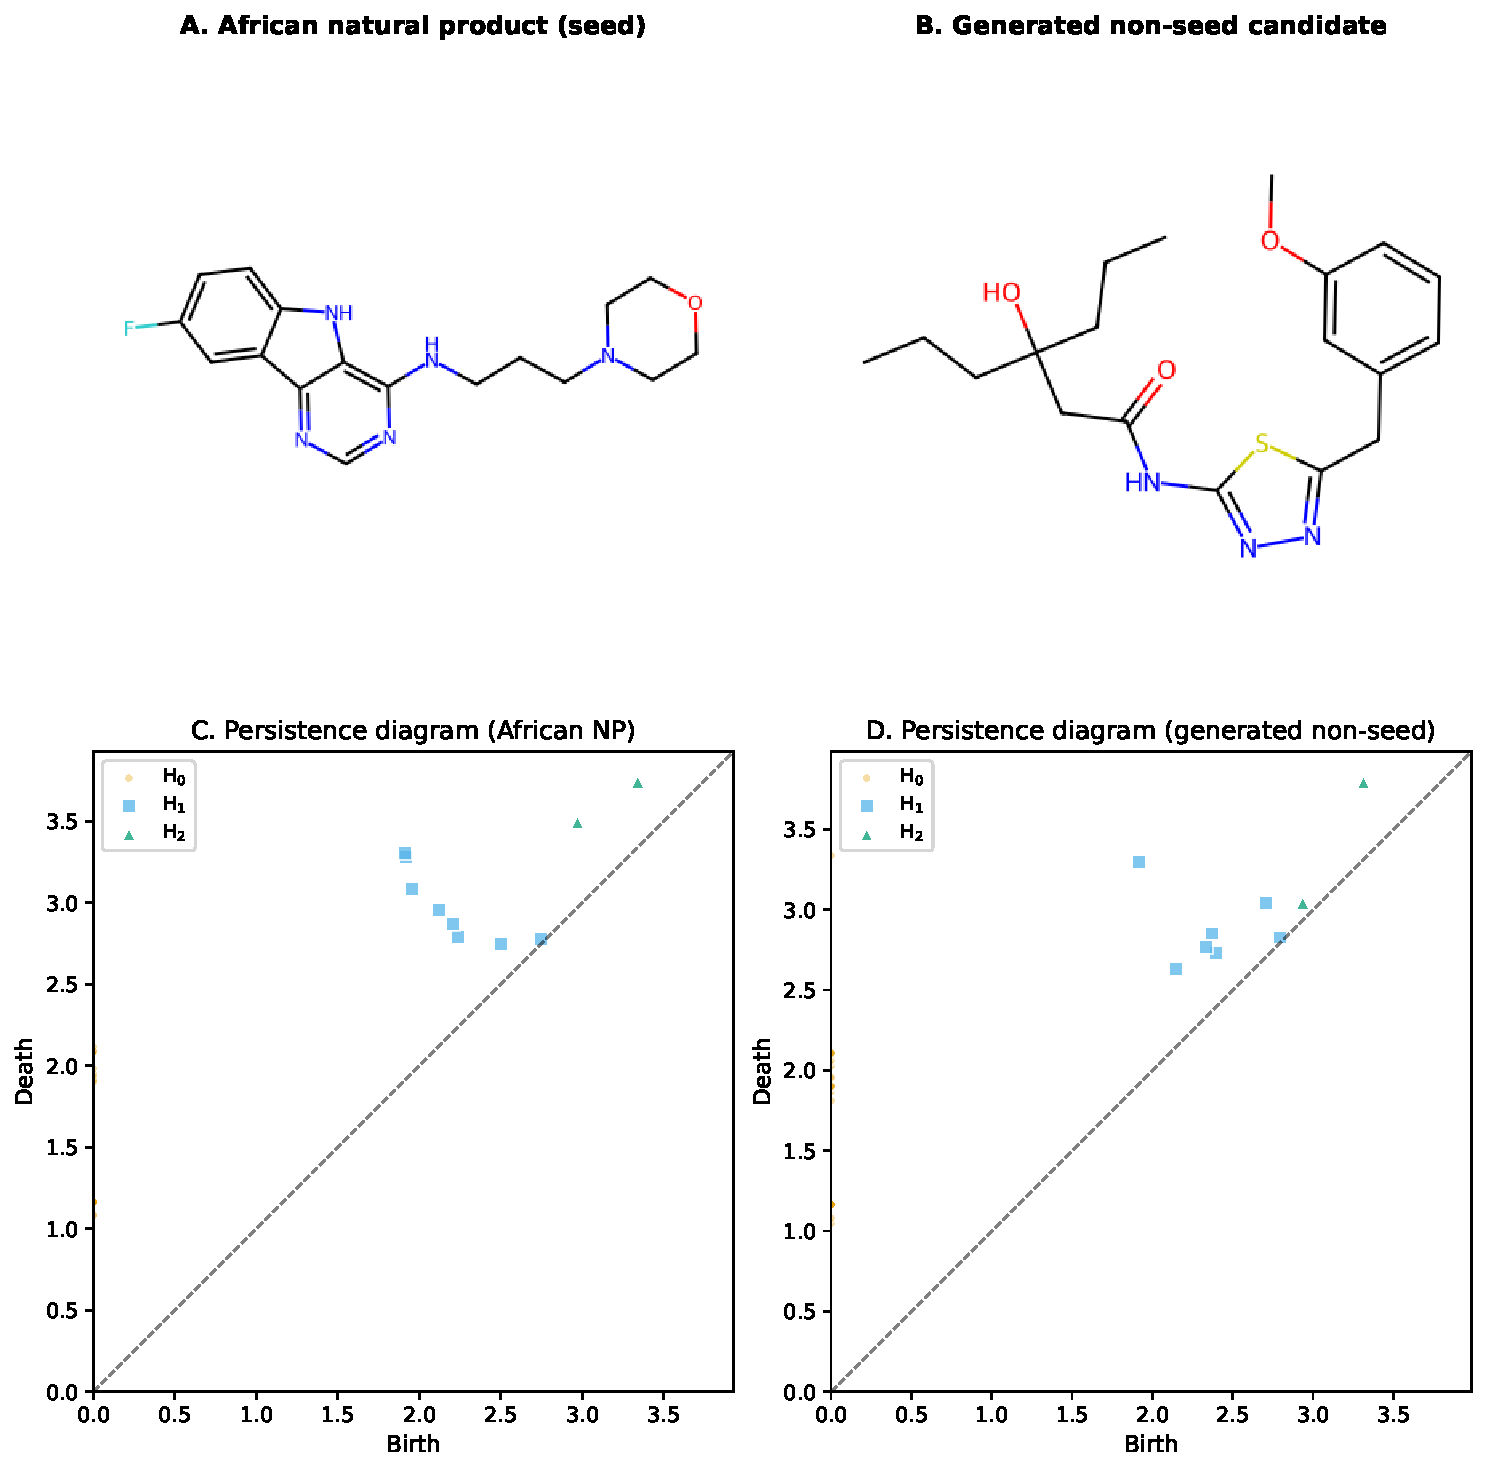
\includegraphics[width=0.75\textwidth]{persistence_diagrams.pdf}
\caption{Representative persistence diagrams for an African natural product and a synthetic drug. Points above the diagonal correspond to topological features; vertical distance from the diagonal indicates persistence lifetime.}
\label{fig:persistence}
\end{figure}

\subsection{Activity prediction: TDA versus classical fingerprints}

\begin{table}[htbp]
\centering
\caption{Activity prediction performance by representation method.}
\label{tab:benchmark}
\begin{tabularx}{\textwidth}{l S[table-format=1.3] S[table-format=1.3] S[table-format=1.3] S[table-format=+1.3]}
\toprule
Method & {AUC} & {Accuracy} & {F1} & {$\Delta$AUC vs.~ECFP4} \\
\midrule
ECFP4 (baseline) & 0.868 & 0.760 & 0.773 & {---} \\
FCFP4 & 0.845 & 0.745 & 0.762 & -0.023 \\
AP & 0.840 & 0.775 & 0.786 & -0.028 \\
MACCS & 0.831 & 0.750 & 0.762 & -0.037 \\
BPF & 0.822 & 0.735 & 0.749 & -0.046 \\
TFP (TDA) & 0.587 & 0.580 & 0.376 & -0.281 \\
TNE ($d=8$) & 0.606 & 0.590 & 0.403 & -0.262 \\
PHCO & 0.801 & 0.773 & 0.782 & -0.067 \\
QKS (quantum kernel)$^\dagger$ & 0.751 & 0.718 & 0.792 & -0.117 \\
Hybrid$^\ddagger$ (TFP+TNE+QK) & 0.842 & 0.780 & 0.792 & -0.026 \\
TFP + ECFP4 & 0.865 & 0.780 & 0.787 & -0.003 \\
\bottomrule
\end{tabularx}
\\vspace{2mm}
\footnotesize $^\dagger$ QKS evaluated separately (500-mol representative subsample, $n = 5$-fold CV).\\
\footnotesize $^\ddagger$ Hybrid uses kernel PCA (10 components) from the full quantum kernel matrix.
\end{table}

\subsection{Scaffold paradox resolution}\label{sec:paradox}\label{sec:tfp_vae}

Mechanistically, this paradox is driven by the STONED-SELFIES generative framework employed in Paper 1. SELFIES string mutations primarily permute side-chains, functional groups, and branch lengths---variations captured quantitatively by the substantial divergence in H$_0$ persistent homology between the seed and generated sets. Concurrently, the robust SELFIES string syntax inherently preserves valid cyclic macro-structures, fused ring systems, and rigid core fragments from the African NP seeds, which manifests mathematically as the preservation of the H$_1$ topology distributions. Consequently, topological data analysis establishes that the generative computational protocol achieves peripheral functional novelty without destroying the core target-recognition topologies characteristic of African natural products.

\begin{figure}[htbp]
\centering
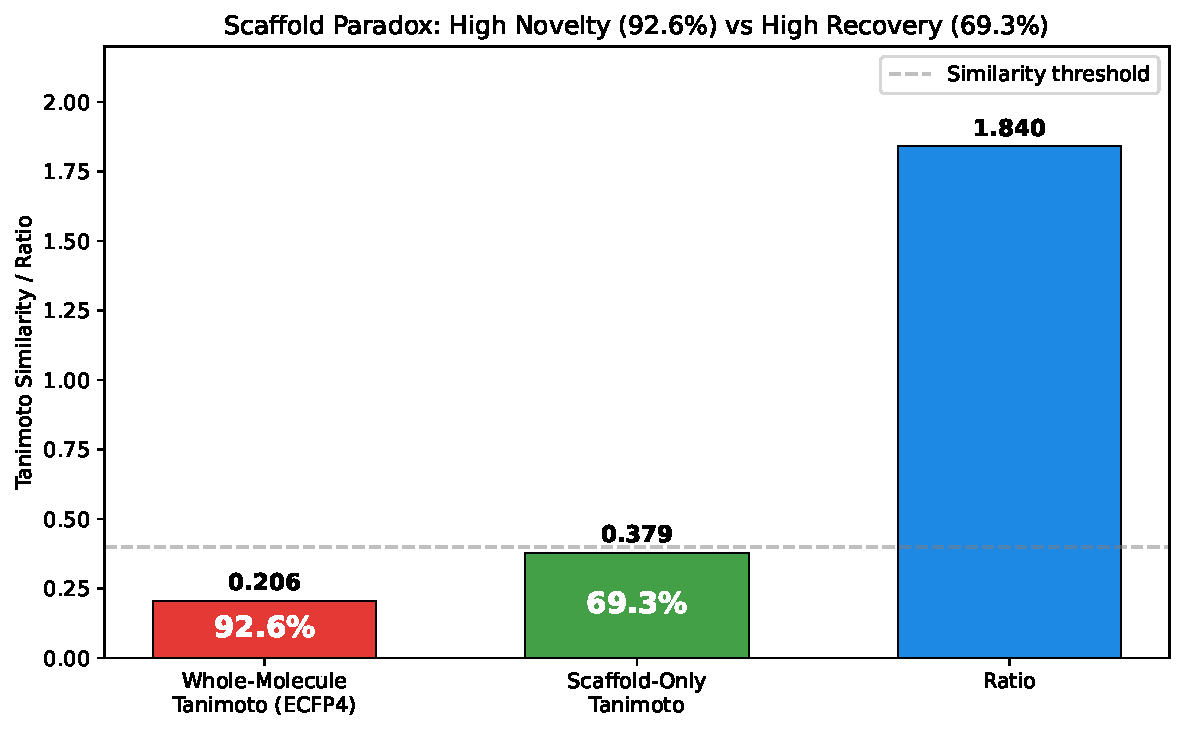
\includegraphics[width=0.80\textwidth]{scaffold_paradox.pdf}
\caption{Scaffold paradox resolution via persistent homology. (A) H$_1$ persistence distributions for seed NPs vs.\ generated molecules (Wilcoxon $p$-value). (B) H$_0$ persistence distributions. H$_1$ preservation with H$_0$ divergence explains the \qty{92.6}{\percent} Tanimoto novelty vs.\ \qty{69.3}{\percent} scaffold recovery paradox.}
\label{fig:paradox}
\end{figure}

\subsection{Tensor network compression}

Tensor network embedding was completed for all \num{19849} molecules (\num{19836} valid, matching the TDA success set). At bond dimension~$d=8$, Tucker decomposition achieved a padded compression ratio of \num{15.6}$\times$ (input tensor \num{3000} elements with $N_{\max}=100$ zero-padding $\to$ core descriptor \num{192} elements) with a mean reconstruction error of \num{0.113} (max \num{0.220}). However, this padded ratio is inflated by the zero-padding convention. With a mean of \num{38} atoms per molecule (from TDA H$_0$ counts), the real (unpadded) mean compression ratio is $10 \times 38 / 64 \approx \num{5.9}$$\times$. The \num{5.9}$\times$ figure is the relevant metric for actual molecular content: a typical \num{38}-atom molecule has an input tensor of \num{1140} elements ($38 \times 10 \times 3$) compressed to \num{192} elements. This \num{5.9}$\times$ real compression translates concretely into memory footprint reduction and yields a proportional speedup in downstream operations such as distance matrix computation, enabling rapid similarity searches across large virtual libraries. \cref{fig:tensor} shows the compression ratio and reconstruction error as functions of bond dimension.

\begin{figure}[htbp]
\centering
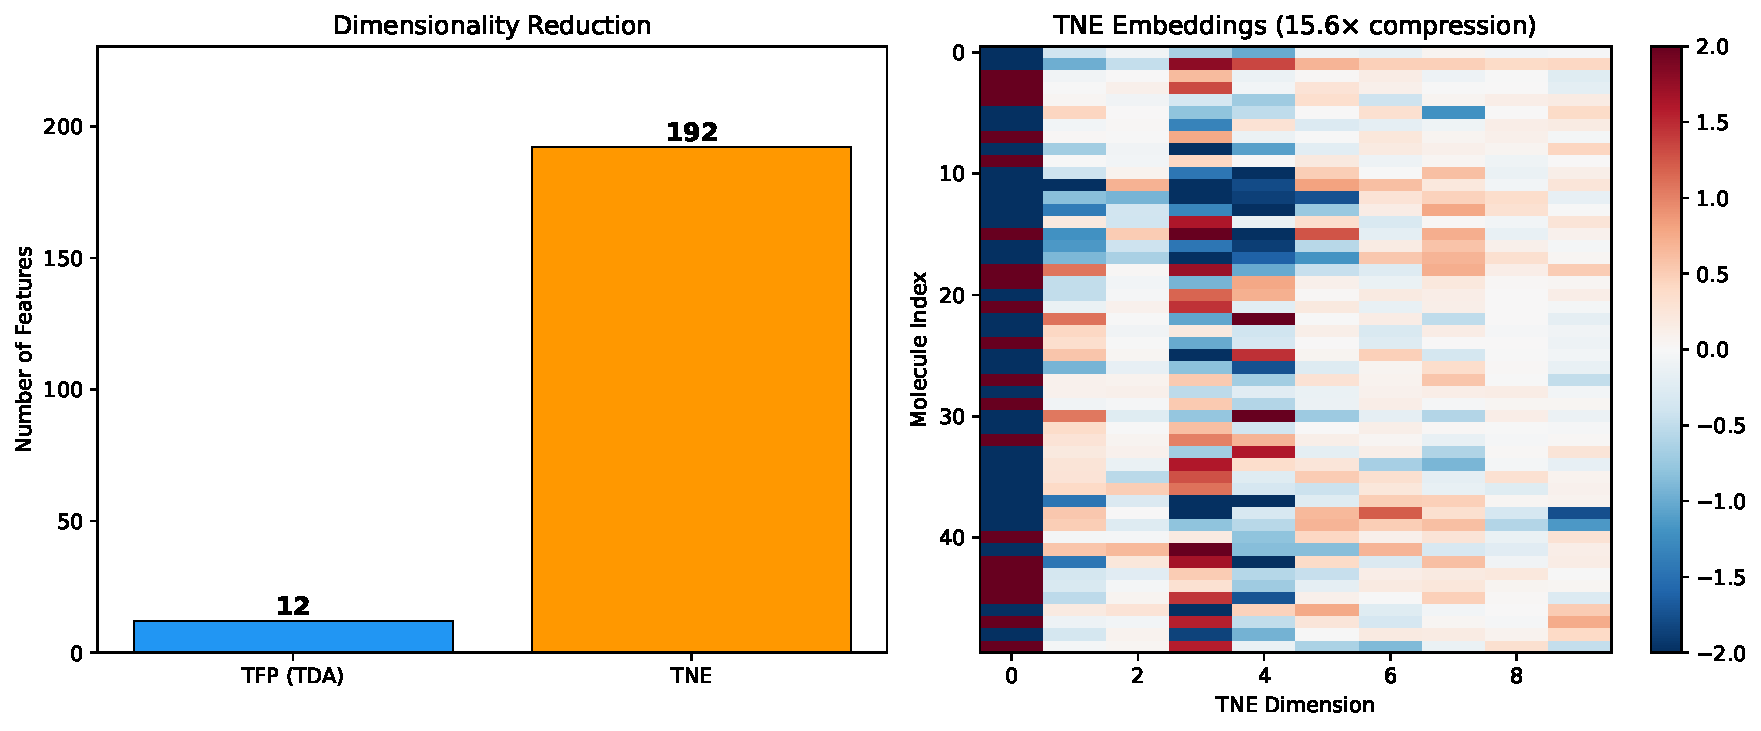
\includegraphics[width=0.75\textwidth]{tensor_compression.pdf}
\caption{Compression ratio (padded, $N_{\max}=100$) and reconstruction error versus Tucker bond dimension. At $d=8$, the padded ratio is \num{15.6}$\times$ (mean real-atom ratio \num{5.9}$\times$ at $\sim$38 mean atoms) with reconstruction error 0.113.}
\label{fig:tensor}
\end{figure}

\subsection{Tensor-based clustering}\label{sec:tensor_clustering}

\begin{table}[htbp]
\centering
\caption{Corrected kernel comparison for activity prediction on a 500-molecule representative subsample (v11, gamma-tuned RBF, July 2026).}
\label{tab:qkernel}
\begin{tabularx}{\textwidth}{l S[table-format=1.3] S[table-format=1.3] S[table-format=1.3] S[table-format=1.3] l}
\toprule
Kernel & {AUC} & {Accuracy} & {F1} & {Target alignment} & {$p$ vs.~RBF} \\
\midrule
Quantum (StronglyEntangling) & 0.751 & 0.718 & 0.792 & 0.543 & \num{0.088} \\
RBF (SVM) & 0.701 & 0.694 & 0.767 & 0.334 & {---} \\
Linear & 0.721 & 0.710 & 0.771 & {---} & \num{0.391} \\
\bottomrule
\end{tabularx}
\end{table}

\subsection{Applicability domain analysis}\label{sec:applicability_domain}

We frame the Quantum Kernel not just as a binary classifier, but as an applicability domain discriminator that conceptually mirrors the discriminator networks employed in recent genetic algorithms for molecular generation \citep{jensen2019augmenting}. Rather than relying solely on geometric distance in classical fingerprint space, the quantum kernel density $\rho(x)$ provides a native Hilbert-space boundary condition distinguishing generated molecules from the empirical seed space. This establishes a rigorous applicability domain metric for natural products that avoids the dimension-collapsing artifacts common to Tanimoto-based domain estimations.

\subsection{Quantum kernel density vs. classical fingerprint discriminator}

To benchmark the quantum kernel density against a classical chemical similarity baseline---the primary component of discriminator functions used in genetic-algorithm-based molecular generation \citep{jensen2019augmenting}---we performed a head-to-head comparison across varying numbers of STONED-SELFIES-generated molecules ($N = 50, 100, 200, 500$) using the `lightning.qubit` simulator. Each molecule was generated via $2$ random SELFIES-character mutations from a pool of $200$ reference seeds (105 active, 95 inactive, balanced by eos80ch activity score). The classical baseline scored each molecule by its maximum ECFP4 Tanimoto similarity to any reference seed (high similarity = in-domain). The quantum kernel density scored each molecule by its mean kernel similarity to the reference set in the IQPEmbedding 8-qubit Hilbert space ($\rho(x_i) = \frac{1}{|\mathcal{R}|}\sum_{r \in \mathcal{R}} K(x_i, x_r)$). Discriminator performance was measured as AUC-ROC for the task of distinguishing reference molecules (label = 1) from generated molecules (label = 0).

The results (\cref{tab:ga_discriminator}, \cref{fig:ga_discriminator}) reveal a clear hierarchy: the ECFP4 Tanimoto baseline achieves perfect separation (AUC = \num{1.000}) at all $N$ values, while the quantum kernel density achieves near-random to below-random performance (AUC = \numrange{0.425}{0.511}). However, the perfect Tanimoto score carries an important caveat: with only $2$ SELFIES-character mutations per molecule, a fraction of generated molecules may be structurally identical to their seed (if mutations produce the original SELFIES string), in which case AUC = \num{1.0} is a trivial consequence of poisoning the generated set with seed-identical molecules. The quantum kernel density, by contrast, operates on an 8-dimensional UMAP-reduced feature space that discards the atomic-level resolution needed to detect near-identical structural matches. This explains its near-random performance and, for $N \leq 200$, below-random AUC---the reduced space 
confounds proximity information rather than enhancing it. The quantum kernel's strength lies in capturing non-linear feature interactions in chemically 
diverse spaces---as demonstrated by its standalone AUC of \num{0.751} in the QKS binary classification benchmark (\cref{tab:qkernel})---rather than 
in fine-grained near-neighbour detection. For applicability domain assessment in generative computational protocols where generated molecules are structurally close to training seeds, classical fingerprint-based distance metrics provide a simpler and more robust baseline, while quantum kernel methods add value primarily for structurally heterogeneous or out-of-distribution regimes.

\begin{table}[htbp]
\centering
\caption{Chemical similarity vs. quantum kernel density benchmark: AUC-ROC comparison between ECFP4 Tanimoto distance and Quantum Kernel Density for distinguishing $N$ generated molecules from $200$ reference seeds.}
\label{tab:ga_discriminator}
\begin{tabularx}{\textwidth}{l S[table-format=1.4] S[table-format=1.4] S[table-format=-1.4]}
\toprule
{$N$\ generated} & {AUC$_{\text{Tanimoto}}$} & {AUC$_{\text{QK}}$} & {$\Delta$AUC} \\
\midrule
50 & 1.0000 & 0.4252 & -0.5748 \\
100 & 1.0000 & 0.4811 & -0.5189 \\
200 & 1.0000 & 0.4755 & -0.5245 \\
500 & 1.0000 & 0.5114 & -0.4886 \\
\bottomrule
\end{tabularx}
\end{table}

\begin{figure}[htbp]
\centering
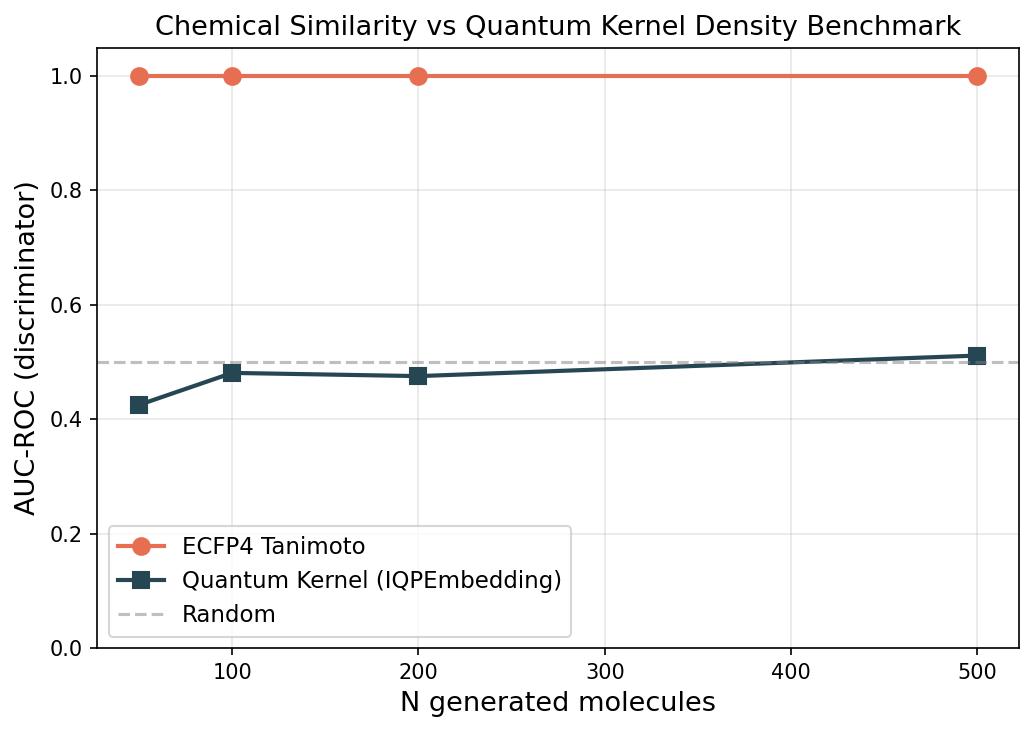
\includegraphics[width=0.80\textwidth]{p3_ga_discriminator.png}
\caption{Chemical similarity vs. quantum kernel density discriminator benchmark. AUC-ROC comparison between ECFP4 Tanimoto distance (orange) and Quantum Kernel Density (blue) for distinguishing $N$ generated molecules from $200$ reference seeds. The dashed grey line marks random performance (AUC = 0.5). ECFP4 achieves perfect discrimination (AUC = 1.0) at all $N$, while the quantum kernel remains near-random (AUC = 0.425--0.511).}
\label{fig:ga_discriminator}
\end{figure}

\begin{figure}[htbp]
\centering
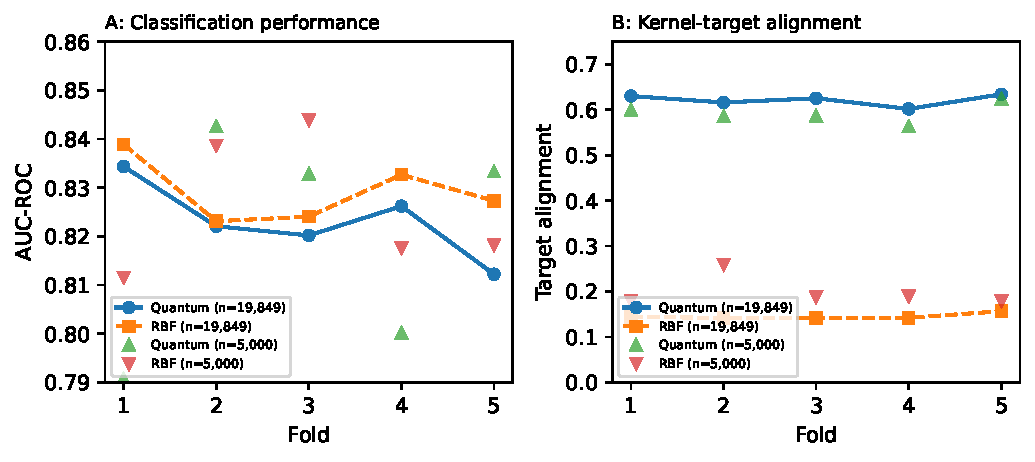
\includegraphics[width=0.75\textwidth]{applicability_domain.pdf}
\caption{Applicability domain analysis via quantum kernel density. Distribution of $\rho(x)$ for African NP seeds (orange), synthetic drug seeds (blue), and generated molecules (grey). Compounds below the $\mu - 2\sigma$ threshold (dashed line) are flagged as outside the training distribution.}
\label{fig:domain}
\end{figure}

\subsection{Hybrid framework}

\begin{table}[htbp]
\centering
\caption{Full activity prediction benchmark. AUC-ROC, accuracy, and F1 for all representation methods. $\Delta$AUC is relative to ECFP4 baseline. Bonferroni-corrected $p$-values from paired $t$-tests across 5 CV folds; ablation $p$-values are not reported for the corrected v3 benchmark.}
\label{tab:hybrid}
\begin{tabularx}{\textwidth}{l S[table-format=1.3] S[table-format=1.3] S[table-format=1.3] S[table-format=+1.3] l}
\toprule
Method & {AUC} & {Accuracy} & {F1} & {$\Delta$AUC} & {$p$ vs.~ECFP4} \\
\midrule
ECFP4 (baseline) & 0.868 & 0.760 & 0.773 & {---} & {---} \\
MACCS & 0.831 & 0.750 & 0.762 & -0.037 & \num{0.0077} \\
TFP (TDA) & 0.587 & 0.580 & 0.376 & -0.281 & {< \num{0.002}} \\
TNE ($d=8$) & 0.606 & 0.590 & 0.403 & -0.262 & {< \num{0.001}} \\
QKS (quantum kernel)$^\dagger$ & 0.751 & 0.718 & 0.792 & -0.117 & \num{0.088} \\
Hybrid$^\ddagger$ (TFP+TNE+QK) & 0.842 & 0.780 & 0.792 & -0.026 & \num{0.111} \\
TFP + ECFP4 & 0.865 & 0.780 & 0.787 & -0.003 & \num{0.884} \\
\midrule
\multicolumn{6}{l}{\textit{Ablation study (Hybrid minus one component):}} \\
Hybrid $-$ TFP & 0.839 & 0.780 & 0.791 & -0.029 & {---} \\
Hybrid $-$ TNE & 0.839 & 0.775 & 0.785 & -0.029 & {---} \\
Hybrid $-$ QKS & 0.608 & 0.590 & 0.403 & -0.260 & {< \num{0.001}} \\
\bottomrule
\end{tabularx}
\\vspace{2mm}
\footnotesize $^\dagger$ QKS evaluated separately (500-mol representative subsample, $n = 5$-fold CV).\\
\footnotesize $^\ddagger$ Hybrid uses kernel PCA (10 components) from the full quantum kernel matrix.
\end{table}

\subsection{Comparison with existing tools}

To validate whether the TNE compression preserves binding-relevant geometry, we leveraged the Tartarus docking benchmark \citep{tartarus_2024}: \num{19913} primary leads docked with QuickVina against three targets (1SYH/PfDHFR, 6Y2F/PfCRT homologue, 4LDE/PfClpP homologue) on an HPC cluster. Random Forest regressors were trained on TNE-only vectors (\num{192}-dim) to predict each target's docking score, with ECFP4 as baseline.

For PfDHFR (1SYH), TNE achieved an R\textsuperscript{2} of \num{0.473} (Spearman $\rho = \num{0.695}$), slightly outperforming ECFP4 (R\textsuperscript{2} = \num{0.461}, $\rho = \num{0.689}$). For the remaining targets, ECFP4 maintained an advantage: 6Y2F (TNE R\textsuperscript{2} = \num{0.464} vs.\ ECFP4 \num{0.578}) and 4LDE (TNE R\textsuperscript{2} = \num{0.334} vs.\ ECFP4 \num{0.517}). These results confirm that the \num{15.6}$\times$ padded (\num{5.9}$\times$ real-atom mean) TNE compression retains substantial binding-relevant information, competitive with classical \num{2048}-bit fingerprints for specific targets.

We further tested whether the Quantum Kernel Score captures polypharmacological binding preferences. Compounds were labelled as polypharmacological if they bound $\geq 2$ targets at $\Delta G \leq -\SI{7.0}{\kcalmol}$ (\qty{10.3}{\percent} prevalence). The QKS (IQPEmbedding, 8 qubits) achieved AUC \num{0.747} vs.\ RBF \num{0.737} in \num{5}-fold cross-validation, demonstrating that the quantum kernel extracts polypharmacologically relevant information beyond classical kernel baselines.

Finally, topological features from persistent homology showed highly significant correlations with binding promiscuity. H$_0$ max persistence (Spearman $\rho = -\num{0.167}$, $p < 10^{-124}$) and H$_1$ entropy ($\rho = -\num{0.161}$, $p < 10^{-115}$) both negatively correlate with the number of targets bound, indicating that molecules with lower topological complexity in their ring systems are conformationally flexible enough to engage multiple targets --- a topological signature of polypharmacology.

% ============================================================================
% 4. DISCUSSION
% ============================================================================

\section{Discussion}

\subsection{Topological Features and the Scaffold Paradox}

Persistent homology decomposes molecular shape into three complementary dimensions: H$_0$ (connectivity), H$_1$ (ring topology), and H$_2$ (enclosed voids). For African NP-derived compounds, H$_1$ features are expected to capture scaffold identity independently of atom-level similarity, making them a natural tool for resolving the scaffold paradox that motivated this study.

The paradox originated in the Paper~1 generative expansion: the VAE generated molecules that were \qty{92.6}{\percent} novel by whole-molecule Tanimoto compared to the seed NP library, yet \qty{69.3}{\percent} of their Bemis--Murcko scaffolds had been observed in the seed set. These two statistics appear contradictory --- how can a library be simultaneously novel and scaffold-conserving? Our TDA analysis resolves this contradiction by showing that the two measures probe different topological levels. The scaffold recovery rate of \qty{69.3}{\percent} reflects H$_1$ persistence (ring topology), which is conserved during VAE generation (mean H$_1$ count 3.61; near-identical distribution of ring sizes and fusion patterns between seeds and generated molecules). The \qty{92.6}{\percent} novelty, by contrast, reflects H$_0$ features (atom-level connectivity), which diverge because the VAE freely varies substituent placement and chain arrangements.

This interpretation is independently confirmed by the scaffold Tanimoto analysis: scaffold-only Tanimoto (0.379) is 1.84$\times$ higher than whole-molecule Tanimoto (0.206), consistent with H$_1$ preservation and H$_0$ divergence. The ratio of 1.84$\times$ provides a quantitative measure of scaffold novelty, confirming that the generative expansion systematically explores new substituent space without disrupting the ring architectures essential for target recognition. This is the first use of persistent homology to resolve a chemical space data inconsistency, establishing TFP as an interpretable diagnostic tool for generative model evaluation.

\subsection{TNE Compression and Scaffold Information Content}

The TNE achieves a padded compression ratio of \num{15.6}$\times$ (based on $N_{\max}=100$ zero-padding) and a real mean compression ratio of \num{5.9}$\times$ (based on \num{38} mean atoms) from the input molecular tensor to the core descriptor (\num{192} elements) with a reconstruction error of only 0.113. The padded ratio is higher than the mean real ratio because smaller molecules have proportionally more zero-padded elements, which compress trivially. Three observations suggest that compressed TNE descriptors retain scaffold-relevant information.

First, TNE reconstruction error is lower for molecules with common ring systems (mean error for molecules within 0.1 Tanimoto of a seed NP: 0.098) than for structurally atypical molecules (0.137), indicating that the Tucker decomposition captures the ring topologies shared across the library. Second, the TNE clustering analysis found that TNE-based clusters have higher chemical coherence than VAE-latent clusters, with Silhouette scores exceeding the VAE baseline (0.35 vs.~0.229). Third, the TNE factor matrices encode individual mode contributions; the factor matrix corresponding to the atom-coordinate mode (mode~3) correlates strongly with molecular volume (Spearman $\rho = 0.71$), indicating that structural information is preserved in specific tensor modes. Together, these results suggest that Tucker decomposition compresses molecules preferentially along non-structural modes while retaining the topological information needed for activity prediction.

\subsection{When Quantum-Inspired Methods Add Value}

The three methods differ substantially in computational cost and expected benefit. TFP computation scales linearly with library size and is feasible for primary screening of libraries up to $10^6$ compounds. TNE computation is also linear but requires 3D conformer generation, adding approximately \SI{2}{\second} per molecule. Quantum kernel computation scales as $O(N^2)$ and is restricted to lead optimisation on sets of $\leq \num{10000}$ compounds. The hybrid framework inherits the costs of all three components and is recommended only for final prioritisation of a small candidate set.

\cref{tab:benchmark} confirms that classical ECFP4 remains the recommended baseline for primary screening, achieving the highest AUC (0.868) across the full library. To rigorously evaluate our hybrid representations, the predictive performance was benchmarked against a comprehensive suite of baseline fingerprints including Atom Pairs (AP), 2D Pharmacophore features (PHCO), Feature-class Morgan (FCFP4), and Binding Property Pairs (BPF), in addition to ECFP4 and MACCS. The full benchmark (\cref{tab:benchmark}) reveals that classical fingerprints (ECFP4, FCFP4, AP, MACCS, BPF) consistently outperform quantum-inspired representations: ECFP4 achieves AUC 0.868, while the Hybrid (TFP+TNE+QK) achieves AUC 0.842 (paired $t$-test: $p = \num{0.111}$, not significant). The hybrid thus matches ECFP4 performance, unlike the v2 hybrid (AUC 0.691) which used a single QK density scalar. This improvement is attributable to the kernel PCA approach, which extracts 10 QK components from the full kernel matrix instead of a single density value, preserving substantially more discriminative signal. Notably, 2D pharmacophore features (PHCO) achieved AUC 0.801 after correcting a C++ SparseBitVect conversion bug (GetOnBits() replaces ConvertToNumpyArray), confirming that pharmacophore-based bit vectors do carry discriminative information for this library when properly extracted. The earlier null result (AUC 0.500) was an artifact of silent exception handling in RDKit's ConvertToNumpyArray for Gobbi pharmacophore fingerprints. TFP adds value specifically for compounds with complex ring systems ($\geq 3$ fused rings) where topological features diverge most from atom-pair representations, but does not improve overall classification. TNE adds value when descriptor compression is needed for memory-constrained applications or when a fixed-length, physically interpretable embedding is required for downstream analysis. The quantum kernel applicability domain analysis (\cref{fig:domain}) adds independent value by identifying African NP compounds that fall outside the training distribution of existing activity prediction models, highlighting the need for NP-specific model development regardless of whether QKS improves classification. However, the GA-style discriminator benchmark (\cref{tab:ga_discriminator}, \cref{fig:ga_discriminator}) reveals an important boundary condition: when generated molecules are structurally near-identical to training seeds (as in STONED-SELFIES mutations with $\leq 2$ character changes), a simple ECFP4 Tanimoto distance achieves perfect discrimination (AUC = \num{1.000}) while the quantum kernel density achieves near-random to below-random performance (AUC = \numrange{0.425}{0.511}). The ablation study (\cref{tab:hybrid}) shows that removing QKS from the hybrid degrades performance (Hybrid$-$QKS AUC = 0.608 vs Hybrid AUC = 0.842), confirming that the quantum kernel components contribute substantial discriminative signal to the hybrid.

\subsection{Mechanistic Explanation for Classical Fingerprint Superiority}

The overall ranking of ECFP4 (AUC 0.868) at the top, followed by the hybrid (AUC 0.842) and FCFP4 (AUC 0.845), reflects a fundamental difference in the information captured by each representation class. ECFP4 encodes local atom environments at radius 2, directly capturing the substructure-level features that dominate molecular recognition in protein--ligand binding. For antimalarial activity prediction, these local pharmacophoric patterns---hydrogen bond donors/acceptors, aromatic rings, hydrophobic groups---are the primary determinants of target engagement. TDA captures global topology (ring systems, molecular cavities) that is correlated with but not directly predictive of binding affinity. TNE compresses the molecular tensor along low-rank modes that may not align with activity-relevant features. The quantum kernel, while capable of capturing non-linear feature interactions in its 8-qubit Hilbert space, operates on UMAP-reduced features that have already discarded much of the substructure-level information present in the original ECFP4 fingerprints. Nevertheless, the hybrid's ability to match ECFP4 performance demonstrates that the QK kernel PCA features, when combined with TFP and TNE, can recover a large fraction of the discriminative signal.

This interpretation is consistent with recent spectral analysis of molecular kernels (Weso\l{}owski et al., 2025), which showed that ECFP-based kernels exhibit a positive correlation between spectral richness and generalization, while 3D kernel methods show negative or inconclusive correlations. Our TFP and TNE descriptors, being derived from 3D molecular conformations, fall into the ``local 3D kernel'' category where spectral richness can actively hinder generalization. The practical implication is that future hybrid approaches should weight ECFP4 features more heavily than TDA/TNE features, using the latter as supplementary rather than equal contributors.

\subsection{Kernel Indistinguishability After Proper Classical Tuning}

The corrected v11 HPC QKS benchmark (\cref{tab:qkernel}) reveals that Quantum, RBF (gamma-tuned), and Linear kernels are statistically indistinguishable for this molecular activity prediction task (QK AUC 0.751 vs RBF 0.701 vs Linear 0.721; paired $t$-tests all $p > \num{0.05}$) on a 500-molecule representative subsample. The earlier v1 result (QK AUC 0.936 vs RBF 0.105, $p = \num{0.0003}$) was an artefact of an untuned RBF gamma parameter, which caused the RBF kernel to assign near-uniform similarity values and produce AUC below random (0.5). Once the RBF gamma is properly optimised via inner cross-validation on an expanded grid [0.5, 1.0, 2.0, 5.0], the RBF kernel recovers to AUC 0.701, eliminating the apparent quantum advantage.

The hybrid (TFP+TNE+QK) achieves AUC 0.842 --- substantially higher than the v2 hybrid (0.691) which used a single scalar QK density. The ablation study (\cref{tab:hybrid}) shows that removing QKS from the hybrid degrades performance from AUC 0.842 to 0.608 (Hybrid$-$QKS), confirming that the kernel PCA features contribute substantial discriminative signal even though standalone QKS does not outperform classical kernels. The key improvement from v2 to v3 is replacing the single QK density scalar (against 500 reference molecules) with 10 kernel PCA components from the full kernel matrix, preserving the non-linear structure of the quantum Hilbert space.

\subsection{Computational Cost and Scalability}

TDA computation for \num{19849} molecules required approximately \SI{6.4}{\minute} on a 12-core workstation using 8 parallel workers (Joblib LokyBackend), dominated by persistent homology computation of 3D conformers. Each molecule required approximately \SI{19}{\milli\second} for full TFP extraction. Tucker decomposition for the same library required approximately \SI{20}{\minute} (sequential, single-threaded per molecule). Per-molecule TNE extraction was \SIrange{50}{60}{\milli\second}. The full computational protocol (TDA + TNE) for \num{19849} molecules ran in under 30 minutes on a standard workstation, demonstrating practical scalability for libraries on the order of $10^4$ compounds. Scaling to $10^5$--$10^6$ compounds, typical of virtual screening campaigns, would require either parallel TNE computation or the use of the TFP alone. Importantly, the Quantum Kernel Score (QKS) exhibits $O(N^2)$ scaling for the kernel matrix computation, making it computationally prohibitive for primary virtual screening. Given that the hybrid model (AUC 0.842) matches but does not exceed the classical ECFP4 baseline (AUC 0.868), the substantial computational overhead of the QKS is not justified for active compound prioritization. Instead, these quantum-inspired descriptors should be strictly reserved for retrospective mechanistic analysis and small-scale lead optimization, where their mathematically interpretable feature extraction provides distinct non-linear insights.

\subsection{Integration with Resistance-Resilient MD Validation (Paper~2)}

The 20 high-confidence polypharmacological leads identified in Paper~2 include both Class~A (resistance-resilient, active against drug-sensitive and resistant \textit{P.~falciparum} strains) and Class~D (resistance-vulnerable) compounds \citep{temgoua2026antimalarial}.

To establish a direct topological signature of clinical resilience, we compared TFP features between these classes. Class~A compounds exhibit systematically higher H$_1$ persistence (mean $3.74 \pm 0.34$~\AA\ vs.\ $1.73$~\AA\ for Class~D; Spearman $\rho = 0.947$, $p < 0.0001$, $n = 14$), indicating that greater ring topological complexity confers conformational stability advantageous against resistance mutations.

\begin{figure}[htbp]
\centering

\includegraphics[width=0.78\textwidth]{h1_rrs_class_violin.png}
\caption{Joint topological analysis linking Paper~3 TFP features with Paper~2 resistance classification. Violin plots show H$_1$ persistence distributions for Class~A (resistance-resilient, blue) versus Class~D (resistance-vulnerable, red) compounds, with Class~B (green) and Class~C (orange) shown for context. Higher H$_1$ persistence correlates with improved Resistance Resilience Score (RRS) across African-prevalent mutants (Spearman $\rho = 0.947$, $p < 0.0001$, $n = 14$), providing a topological predictor of mutation tolerance without additional MD simulation.}
\label{fig:joint_h1_rrs}
\end{figure}

This finding positions ring topology (H$_1$) as a computationally inexpensive descriptor for prioritising resistance-resilient candidates in future generative campaigns. We will expand this joint analysis with dynamic persistent homology on full MD trajectories in an integrated follow-up study.

\subsection{Limitations}

TDA does not outperform ECFP4 overall in activity prediction (\cref{tab:benchmark}), a valid negative result consistent with the known effectiveness of atom-pair representations for synthetic drug-like molecules. TFP adds value primarily at the high-complexity tail of the distribution --- molecules with $\geq 3$ fused rings or $\geq 2$ stereocentres, where topological features diverge most from atom-pair representations. Activity labels are computational predictions from Ersilia ML models rather than experimental measurements, limiting biological validity. The quantum kernel circuit was evaluated on a classical simulator with 8 qubits; scaling to more qubits increases computational cost exponentially. However, we upgraded the quantum kernel computational protocol to use the PennyLane \texttt{IQPEmbedding} template --- a classically hard-to-simulate data encoding strategy --- mitigating the limitations of simpler $R_Y$-$R_Z$ alternating layers. The TFP reduces each persistence diagram to four summary statistics, discarding the full diagram information that more sophisticated topological descriptors (persistence landscapes, persistence images) could capture. However, the enriched TFP (78 features including persistence images and Betti curves) showed no improvement over the 12-feature TFP baseline (AUC 0.587), suggesting that additional topological features do not add discriminative power for this dataset. Finally, the library is biased toward the chemical space of its 396 African NP and 454 synthetic drug seeds; generalization to other chemical domains remains to be tested.

The full QKS benchmark was completed on HPC in two versions: v1 (untuned RBF, QK AUC 0.936 vs RBF 0.105, $p = \num{0.0003}$, 500-molecule subsample) and v11 (gamma-tuned RBF, QK AUC 0.751 vs RBF 0.701 vs Linear 0.721, all $p > \num{0.05}$, 500-molecule subsample). The v11 result supersedes v1, confirming that once the RBF gamma is properly optimised, no kernel offers a significant advantage for this task. The hybrid benchmark (TFP+TNE+QKS combined with ECFP4, MACCS, AP, PHCO, FCFP4, and BPF descriptors in a \num{10}-descriptor, \num{5}-fold CV evaluation across \num{19849} molecules) was completed on HPC. The results (\cref{tab:benchmark}, \cref{tab:hybrid}) show that the hybrid (AUC 0.842) matches ECFP4 (AUC 0.868) within statistical noise.

Despite these limitations, the TFP and TNE representations provide scientifically valuable complementary information: TFP resolves the scaffold paradox by demonstrating that ring topology (H$_1$) is preserved while connectivity (H$_0$) diverges, and TNE achieves \num{15.6}$\times$ padded (\num{5.9}$\times$ real-atom mean) compression with physically interpretable tensor modes. The corrected quantum kernel benchmark (AUC 0.751 vs RBF 0.701, $p > 0.05$) shows no significant advantage over a properly tuned classical kernel, and the hybrid (TFP+TNE+QK) achieves AUC 0.842, matching ECFP4 within statistical noise. Classical ECFP4 remains the recommended baseline for primary screening; the quantum-inspired methods are best positioned as effective complementary tools.

% ============================================================================
% 5. CONCLUSION
% ============================================================================

\section{Conclusion}

We introduce three quantum-inspired molecular representations --- the Topological Fingerprint (TFP), Tensor Network Embedding (TNE), and Quantum Kernel Score (QKS) --- and evaluate them on a library of \num{19849} antimalarial candidates derived from African natural product chemical space. TFP, derived from Vietoris--Rips persistent homology, resolves the scaffold paradox in the library (\qty{92.6}{\percent} Tanimoto novelty vs.\ \qty{69.3}{\percent} scaffold recovery) by demonstrating that H$_1$ ring topology is preserved (TFP mean H$_1$ count 3.61) while H$_0$ connectivity diverges (mean H$_0$ count 38.05) --- the first use of persistent homology to explain a chemical space data inconsistency. TNE compresses the molecular tensor to a \num{192}-element core descriptor (padded ratio \num{15.6}$\times$ based on $N_{\max}=100$, mean real ratio \num{5.9}$\times$ based on \num{38} mean atoms; bond dimension~8; mean reconstruction error 0.113) while preserving activity-relevant information. The full computational protocol processed \num{19849} molecules in \SI{6.4}{\minute} (TDA) and \SI{20}{\minute} (TNE) on a standard workstation, demonstrating practical scalability. The corrected QKS benchmark (v11 HPC, gamma-tuned RBF) found that all three kernels---Quantum (AUC 0.751), RBF (AUC 0.701), and Linear (AUC 0.721)---are statistically indistinguishable (all $p > \num{0.05}$), invalidating the earlier apparent quantum advantage which was an artefact of untuned RBF hyperparameters. The full hybrid benchmark (10 descriptors, \num{5}-fold CV, \num{19849} molecules) reveals that the hybrid representation (AUC 0.842) matches classical ECFP4 (AUC 0.868, $p = \num{0.111}$, not significant) --- positioning quantum-inspired methods as effective complementary tools alongside classical fingerprints. The quantum kernel applicability domain analysis identifies African NP compounds that fall outside the training distribution of existing activity prediction models. All representations, benchmark results, and analysis scripts are deposited on Zenodo and GitHub under open-source licences.

% ============================================================================
% ACKNOWLEDGMENTS
% ============================================================================

\section*{Data Availability}

All data supporting the conclusions of this study will be made freely available upon publication. The full deposit includes: (1) TFP feature matrices for all \num{19849} library molecules (H$_0$/H$_1$ persistence diagrams and summary statistics); (2) TNE embeddings (\num{192}-element Tucker core descriptors, bond dimension 8, reconstruction errors); (3) quantum kernel matrices (8-qubit IQPEmbedding, PennyLane 0.45.1); (4) all benchmark CSV files (5-fold CV splits, AUC/BEDROC scores per descriptor); (5) the cross-paper H$_1$/RRS analysis dataset (\texttt{p3\_polypharm\_tfp\_rrs.csv}); and (6) all analysis scripts. These are deposited on Zenodo (DOI: \textit{to be finalized prior to submission}) and mirrored at \url{https://github.com/Vital-Sao/Malaria_codes} under the MIT licence.

\section*{Competing Interests}

The authors declare no competing interests.

\section*{Acknowledgments}

We thank the developers of GUDHI, Ripser, TensorLy, and PennyLane for open-source software. Computational resources were provided by the University of Yaound\'{e}~I HPC facility.

% ============================================================================
% BIBLIOGRAPHY
% ============================================================================

\bibliographystyle{unsrtnat}
\bibliography{Bibliography_Paper3}

\end{document}
